\documentclass{article}

\usepackage[final]{nips_2017}

\usepackage{ctex}
\usepackage{hyperref}
\usepackage{multirow}
\usepackage{xcolor}
\usepackage{minted}
\usepackage{amsmath,amsfonts}
\usepackage{graphicx}
\usepackage{pgfplots}
\usepackage{romannum}
\usepackage{nicefrac}

\usetikzlibrary{arrows,automata}

\title{《计算机组成原理》大作业实验报告}
\author{
    张蔚\\
    计算机科学与技术系\\
    清华大学\\
    \texttt{zhangwei15@mails.tsinghua.edu.cn}
    \And
    张蒲石\\
    计算机科学与技术系\\
    清华大学\\
    \texttt{zhangps15@mails.tsinghua.edu.cn}
    \And
    赵嘉霖\\
    计算机科学与技术系\\
    清华大学\\
    \texttt{zhao-jl15@mails.tsinghua.edu.cn}
}
\date{\today}

\begin{document}

\pagenumbering{roman} % Start roman numbering
\maketitle
\tableofcontents
\newpage
\pagenumbering{arabic} % Switch to normal numbers

\section{实验概述}

\subsection{实验目标}

本次实验的基本目标是,在 ThinPAD 教学实验平台上,实现能够执行给定的$30$条指令的CPU。
并且该 CPU 应当能够正常运行给出的监控程序和$5$个测试程序。
我们需要实现的$30$条指令如表 \ref{tab:instruction}。
\begin{table}[ht]
\centering
\caption{基本指令与扩展指令}
\label{tab:instruction}
\begin{tabular}{|c|l|l|l|l|l|}
\hline
& \texttt{ADDIU} & \texttt{ADDIU3} & \texttt{ADDSP}  & \texttt{ADDU} & \texttt{B}    \\ \cline{2-6}
& \texttt{BEQZ}  & \texttt{BNEZ}   & \texttt{BTEQZ}  & \texttt{CMP}  & \texttt{JR}   \\ \cline{2-6}
& \texttt{LI}    & \texttt{LW}     & \texttt{LW\_SP} & \texttt{MFIH} & \texttt{MFPC} \\ \cline{2-6}
& \texttt{MTIH}  & \texttt{MTSP}   & \texttt{NOP}    & \texttt{OR}   & \texttt{AND}  \\ \cline{2-6}
\multirow{-5}{*}{基本指令} & \texttt{SRA} & \texttt{SUBU} & \texttt{SW} & \texttt{SW\_SP} & \texttt{SLL} \\ \hline
扩展指令 & \textcolor{red}{\texttt{BTNEZ}} & \textcolor{red}{\texttt{NEG}} & \textcolor{red}{\texttt{SLTI}} & \textcolor{red}{\texttt{SLTUI}} & \textcolor{red}{\texttt{SRLV}} \\ \hline
\end{tabular}
\end{table}

\subsection{实验成果}

经过三星期的奋战,我们的最终成果如下:
\begin{enumerate}
    \item 支持$5$级指令流水的 CPU,能够执行25条基本指令和5条扩展指令;
    \item 正确处理流水线中的冲突,延迟槽行为和提供的模拟器一致;
    \item 实现了 VGA 扩展,能够输出$80 \times 30$的字符阵列或预先烧制好的位图;
    \item 实现了键盘扩展,能够正常接收除小键盘和功能键以外的按键;
    \item 实现了 Flash 自启动功能,能够自动装载预先导入 Flash 的程序。
\end{enumerate}
此外,我们还基于以上功能实现了两个应用程序:
\begin{enumerate}
    \item 利用$16$位定点数实现的神经网络手写数字识别程序;
    \item 利用$80 \times 30$字符阵列实现的 PowerPoint 程序。
\end{enumerate}

\section{总体设计}

为了降低实现的复杂度,我们将 CPU 和内存控制模块分开实现,按照一般的习惯,以下称内存控制器为 NorthBridge。
我们在本小节中将先介绍 CPU 的设计,然后讨论 NorthBridge 的实现。
我们会着重解释设计的思路和缘由而尽量避免罗列代码。

\subsection{CPU}

我们的 CPU 采用了 RISC 中经典的$5$级流水结构,五个阶段分别为 Instruction Fectch (IF),Instruction Decode (ID),Execution (EXE),Memory (MEM),Write Back (WB)。

\subsubsection{数据通路}

图 \ref{fig:datapath} 为我们在CPU设计阶段画出的数据通路示意图(可直接放大查看)。

\begin{figure}[ht]
\centering
\includegraphics[width=\textwidth]{datapath.pdf}
\caption{数据通路示意图}
\label{fig:datapath}
\end{figure}

图 \ref{fig:datapath} 中的每一个模块都对应一个 VHDL Entity,其中左侧为输入信号,右侧为输出信号。
由于我们只使用了 VHDL 中的 \mintinline{vhdl}{STD_LOGIC} 和 \mintinline{vhdl}{STD_LOGIC_VECTOR},因此不再标出数据类型。

从图中可以看出,CPU接收的输入和输出有:
\begin{itemize}
    \item \mintinline{vhdl}{Clock : in STD_LOGIC} CPU 时钟信号;
    \item \mintinline{vhdl}{Reset : in STD_LOGIC} CPU 复位信号;
    \item \mintinline{vhdl}{InstAddress : out STD_LOGIC_VECTOR(15 downto 0)} 指令地址;
    \item \mintinline{vhdl}{InstData : in STD_LOGIC_VECTOR(15 downto 0)} 指令数据;
    \item \mintinline{vhdl}{DataAddress : out STD_LOGIC_VECTOR(15 downto 0)} 读写内存地址;
    \item \mintinline{vhdl}{DataInput : in STD_LOGIC_VECTOR(15 downto 0)} 从内存读出的数据;
    \item \mintinline{vhdl}{DataOutput : out STD_LOGIC_VECTOR(15 downto 0)} 希望写入内存的数据;
    \item \mintinline{vhdl}{MemReadEN : out STD_LOGIC} 内存读使能;
    \item \mintinline{vhdl}{MemWriteEN : out STD_LOGIC} 内存写使能。
\end{itemize}

容易看出,除了 \mintinline{vhdl}{Clock : STD_LOGIC} 和 \mintinline{vhdl}{Reset : STD_LOGIC} 外,CPU 只需要和内存进行交互。
这一事实为通过 NorthBridge 将 CPU 从系统中隔离出来提供了可能。

在此基础上,新加入的外部设备只需要和 NorthBridge 交互,而 CPU 通过 Memory-mapped I/O (MMIO) 即可操作它们。

\subsubsection{寄存器编址}

首先观察和特殊寄存器相关的指令,如 \texttt{MTSP R0},一个等价但汇编器不接受的写法是 \texttt{ADDIU3 R0 SP 0x0}。
本质上看,特殊寄存器和通用寄存器都实现了存储一个字的功能,如果我们能够对它们一视同仁,那么在 ID 段就可以对前一种指令生成后一种指令的控制信号。
如此一来,就不需要为跟特殊寄存器相关的指令专门设计电路。

因此,我们使用一个$16 \times 16\texttt{bit}$的片上内存实现寄存器文件,每个寄存器都对应一个$4$位的地址,对应关系见 \href{run:./Instructions.xlsx}{Instructions.xlsx},此处不再罗列。

另外要注意的是片上内存应当使用下降沿触发,这样可以实现``前半周期写入,后半周期读出''的功能。

\subsubsection{结构冲突}\label{sec:conflict}

为了方便实现,我们的 CPU 不考虑访问指令内存时的结构冲突,这种结构冲突将由NorthBridge解决,见 \ref{sec:memory} 小节。

\subsubsection{数据冲突}

对于不涉及内存访问的数据冲突,我们使用一个旁路单元,能够把 MEM 或 WB 段的运算结果直接传递到 EX 段。
对于涉及到内存访问的数据冲突,若前一条为 LW 指令,后一条立即用到 LW 指令要写回的寄存器,我们会在 EX 段插入空泡,将运算延迟一个时钟周期。

\subsubsection{控制冲突}

在 ID 段,我们会根据解码的指令进行 PC 寄存器的更新。
对于 B 型的指令,我们会使用分支预测单元进行分支预测,详情见 \ref{sec:branch-prediction} 小节;
而对于 J 型指令,我们总是选择不跳转,之后进入 EX 段时直接当做分支预测失败处理;
对于其余指令,将 PC 值加一即可。

遇到 J 型指令总不跳转的理由有:
\begin{itemize}
    \item J 型指令涉及到从寄存器中取目标地址,因此可能会引发数据冲突;
    \item 为了应对数据冲突而加入从 MEM 或 WB 段到 ID 段的旁路单元太过复杂;
    \item J 型指令不常出现,而且每次只会引起一个周期的损失。
\end{itemize}

对于预测失败的分支或跳转指令,我们会清空 IF/ID 阶段寄存器并更新 PC 寄存器为正确值。

\subsection{内存控制}\label{sec:memory}

\ref{sec:conflict} 小节中已经提到,CPU的结构冲突将交给NorthBridge解决,本小节中我们将详细介绍NorthBridge的工作方式。

首先,为了简化实现,我们只将 RAM2 作为内存使用,即指令和数据存放在同一片内存上。
这样一来,在一个 CPU 时钟周期内,NorthBridge 需要完成两次仿存才能满足 CPU 的需求。
因此,我们为 NorthBridge 模块设计了一个三状态的状态机,如图 \ref{fig:state-machine}。

\begin{figure}[ht]
\centering
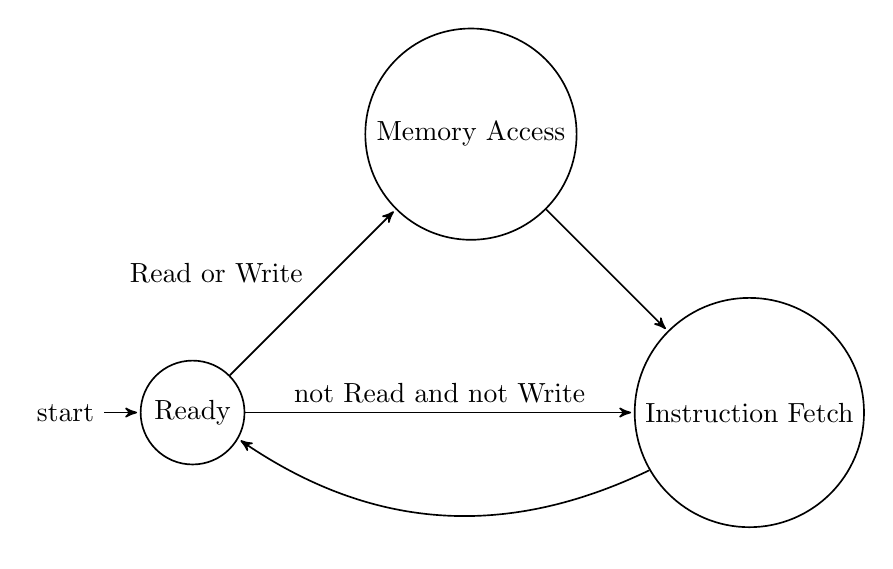
\begin{tikzpicture}[->,>=stealth',shorten >=1pt,auto,node distance=5cm,semithick]
  \node[initial,state] (A)                    {Ready};
  \node[state]         (B) [above right of=A] {Memory Access};
  \node[state]         (C) [below right of=B] {Instruction Fetch};

  \path (A) edge             node {Read or Write} (B)
            edge             node {not Read and not Write} (C)
        (B) edge             node {} (C)
        (C) edge [bend left] node {} (A);
\end{tikzpicture}
\caption{NorthBridge状态机}
\label{fig:state-machine}
\end{figure}

图 \ref{fig:state-machine} 中转移边上的 Read 和 Write 对应着内存的读写使能信号,未标明转移条件则表明总是无条件转移。
各个状态的功能如下:
\begin{itemize}
    \item Ready 状态一方面给 NorthBridge 判断下一步应该转移到哪个状态提供机会,另外还起到了给 Memory Access 中的写操作提供数据准备时间的作用;
    \item Memory Access 状态下会从内存中读取数据或向内存中写入数据;
    \item Instruction Fetch 状态下会从内存中读取下一条指令。
\end{itemize}

在 Ready 状态时我们会将 CPU 时钟信号拉低,另外两个状态将 CPU 时钟信号拉高。
由此可知,当没有访存操作时,CPU 时钟频率为 NorthBridge 频率的 $\frac{1}{2}$;当有仿存操作时,CPU 时钟频率为 NorthBridge 频率的 $\frac{1}{3}$。

我们根据要求将串口的数据和状态映射到 \texttt{0xBF00} 和 \texttt{0xBF01} 两个地址上,另外显存和键盘都做了类似的映射,将在 \ref{sec:vga} 和 \ref{sec:keyboard} 小节中介绍。

\section{性能优化}

本小节中,我们将会对 CPU 实现中的性能优化做简要介绍,并给出测试程序的运行结果。

\subsection{分支预测}\label{sec:branch-prediction}

由于我们采用了模块化设计,因此一开始并没有加入分支预测模块。
根据我们的观察,在引入分支预测模块后,在测试程序上的表现大概有$30\%$的提升。
前面已经提到,我们只考虑对 B 型指令的分支预测,我们为此使用了深度为$16$的 Branch History Buffer (BHB)。

我们使用 PC 寄存器的低$4$位作为 BHB 的索引,BHB 中每项为$2\texttt{bit}$的计数器,表示一个四状态的状态机,如图 \ref{fig:counter}。
约定状态的高位为$1$时跳转,高位为$0$时不跳转,预测正确为 hit,预测错误为 miss。

\begin{figure}[ht]
\centering
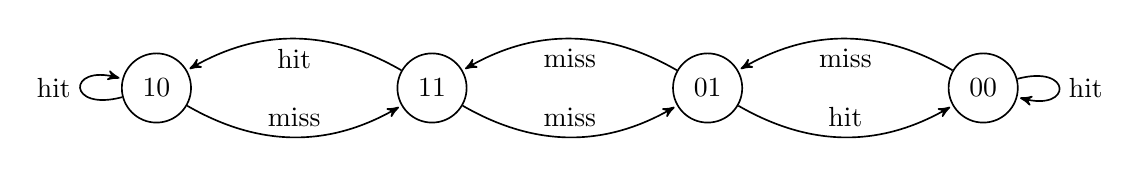
\begin{tikzpicture}[->,>=stealth',shorten >=1pt,auto,node distance=3.5cm,semithick]
  \node[state] (A)              {$10$};
  \node[state] (B) [right of=A] {$11$};
  \node[state] (C) [right of=B] {$01$};
  \node[state] (D) [right of=C] {$00$};

  \path (A) edge [loop left]  node {hit} (A)
            edge [bend right] node {miss} (B)
        (B) edge [bend right] node {hit} (A)
            edge [bend right] node {miss} (C)
        (C) edge [bend right] node {miss} (B)
            edge [bend right] node {hit} (D)
        (D) edge [bend right] node {miss} (C)
            edge [loop right] node {hit} (D);
\end{tikzpicture}
\caption{BHB中表项表示的状态机}
\label{fig:counter}
\end{figure}

我们一开始使用了大小为$256$的 BHB,由于给出的测试程序较短,因此我们将 BHB 大小改为$16$以减少综合时间。
实际测试显示 CPU 性能未受影响。

\subsection{CPU变频}

由于我们采用了 CPU 为内存频率二分或三分频的设计,提高内存频率成为提高运行速度的最直接方法。
我们使用 ISE 提供的 Digital Clock Manager (DCM) 进行了反复测试。
我们发现,在关闭ISE优化的情况下,内存频率能够达到$83\texttt{MHz}$左右,此时对应的CPU频率在无访存时约为$41.5\texttt{MHz}$,在有访存时约为$27.7\texttt{MHz}$。
一旦频率上升到$85\texttt{MHz}$,就会经常出现访存错误,进而导致监控程序无法运行。

\subsection{测试结果}

我们使用$83.3\texttt{MHz}$时钟进行测试,第一至第五个测试程序的运行结果如图 \ref{fig:result}。

\begin{figure}[ht]
\centering
\includegraphics[width=\textwidth]{figures/result.png}
\caption{测试程序运行结果}
\label{fig:result}
\end{figure}

由此可计算出实际运行的平均频率如表 \ref{tab:performance} 所示,从表格前三行可以看出我们的分支预测相当有效,很大程度上挽回了分频引起的性能损失。
而在第四个程序中,由于大量的仿存操作和数据冲突,使得 CPU 的频率降到了最低。

\begin{table}[ht]
\centering
\caption{测试结果}
\label{tab:performance}
\begin{tabular}{|c|c|c|c|}
\hline
测试程序序号 & 指令条数(百万条) & 运行时间(\texttt{s}) & 平均频率(\texttt{MHz}) \\ \hline
$1$      & $150$       & $3.625$   & $41.38$     \\ \hline
$2$      & $225$       & $5.422$   & $41.50$     \\ \hline
$3$      & $100$       & $2.437$   & $41.03$     \\ \hline
$4$      & $150$       & $5.429$   & $27.63$     \\ \hline
$5$      & $75$        & $2.127$   & $35.26$     \\ \hline
\end{tabular}
\end{table}

\section{扩展功能}

\subsection{VGA}\label{sec:vga}

对于VGA模块,根据应用程序的需求,我们分别实现了$80 \times 30$的字符阵列显示功能和基于位图的手写数字显示,下面分别进行介绍。

\subsubsection{字符阵列显示}

我们使用一个$2048 \times 8$的 ROM 存放 \texttt{0x00}---\texttt{0x7F} 这$128$个字符的位图,下面给出一段代码来直观地说明 ROM 的数据组织方式。

\begin{minted}[mathescape=true]{vhdl}
constant ADDR_WIDTH : INTEGER := 11;
constant DATA_WIDTH : INTEGER := 8;

type ROM_TYPE is array (0 to 2**ADDR_WIDTH-1)
    of STD_LOGIC_VECTOR(DATA_WIDTH-1 downto 0);

-- ROM definition
constant ROM : ROM_TYPE := ( -- $2^{11} \times 8$
    -- ......
    -- code 0x7b
    "00000000", -- 0
    "00000000", -- 1
    "00001110", -- 2     ***
    "00011000", -- 3    **
    "00011000", -- 4    **
    "00011000", -- 5    **
    "01110000", -- 6  ***
    "00011000", -- 7    **
    "00011000", -- 8    **
    "00011000", -- 9    **
    "00011000", -- a    **
    "00001110", -- b     ***
    "00000000", -- c
    "00000000", -- d
    "00000000", -- e
    "00000000", -- f
    -- ......
);
\end{minted}

我们的 VGA 模块使用$640 \times 480$的分辨率,每个字符大小$8 \times 16$,因此我们准备了一块大小为$128 \times 32 \times 8\texttt{bit}$的字符显存,对应内存地址 \texttt{F000}---\texttt{FFFF},当然字符显存中只有$80 \times 30 \times 8\texttt{bit}$是可显示的区域。
写其中一个地址相当于将写数据的低$8$位写入字符显存,若该数据的低$8$位对应了一个可见字符的 ASCII 码,则会在屏幕对应位置显示一个字符。

具体的显示过程如图 \ref{fig:font},根据一个像素的$x$和$y$坐标计算对应字符阵列中的行号和列号,访问字符显存并取出对应位置的 ASCII 码。
然后根据 ASCII 码访问 ROM,此时会取出 ROM 中对应字符的某一行,再使用$x$坐标从这行的$8$个位中取出一位,最后输出到屏幕对应像素上。

\begin{figure}[ht]
\centering
\includegraphics[width=\textwidth]{figures/font.png}
\caption{字符显示过程示意图}
\label{fig:font}
\end{figure}

我们在这里遇到的一个问题是,字符显存要过一个周期才能输出结果,因此显示时总是有一个像素的偏移量。
我们发现将字符显存接上$50\texttt{MHz}$时钟而不是 VGA 的$25\texttt{MHz}$时钟即可,这时 VGA 的一个周期对应字符显存的两个周期,因而不存在上述问题。

\subsubsection{手写数字显示}

% \subsection{Flash}

\subsection{键盘}\label{sec:keyboard}

由于键盘按下和松开会产生三组串行数据,我们每次只记录 BREAK 信号后的一组数据,即按键松开后的第二组串行数据。
如此一来可以避免繁琐的判断和处理过程。
另外从键盘获得的扫描码并不是对应按键的 ASCII 码,因此我们使用了一块 ROM 完成从扫描码到 ASCII 的映射。
我们将 \texttt{0xBF02} 和 \texttt{0xBF03} 分别映射到键盘的数据位和状态位上,获取输入字符的方法类似于串口的读操作。

\subsection{Flash}

由于我们只需要实现读Flash的功能,因此Flash模块实现较为容易,参考实验指导书中给出的描述即可,此处不再赘述。

\section{应用程序}

\subsection{手写数字识别}

\begin{figure}[ht]
\centering
\includegraphics[width=\textwidth]{figures/mnist.png}
\caption{手写数字识别程序运行结果}
\label{fig:mnist}
\end{figure}

我们为实现这个应用程序,完成了以下工作:
\begin{itemize}
    \item 使用 Python 实现神经网络训练,并将网络权重转换为$16$位定点数,代码见 \href{run:./utils/mlp}{utils/mlp/};
    \item 实现手写数字的 VGA 显示模块;
    \item 使用汇编实现神经网络的前向传播部分,代码见 \href{run:./utils/neural_network.asm}{utils/neural\_network.asm}。
\end{itemize}

如图 \ref{fig:mnist} 所示,图中左侧为当前输入的图片,右侧的对钩为神经网络的预测值,详情可见演示视频 \href{run:.}{mnist.mp4}。

另外,我们使用该网络对整个 MNIST 数据集进行了测试。
我们发现,即便是使用$16$位定点数,该网络在测试集上的精度仍然能够达到$92\%$左右。

\subsection{PowerPoint}

\begin{figure}[ht]
\centering
\includegraphics[width=\textwidth]{figures/ha.png}
\caption{PowerPoint程序运行照片}
\label{fig:ppt}
\end{figure}

在实现这个程序时,我们充分利用了之前完成的$80 \times 30$字符阵列显示功能,将 PPT 的内容以字符画的形式展现到屏幕上。
用户在使用时需要先准备好字符形式的 PPT 然后再将 PPT 的内容烧写进内存,实际效果如图,详情可见演示视频 \href{run:.}{ppt.mp4}。

控制 PPT 播放的程序见 \href{run:utils/pointless.asm}{utils/pointless.asm},示例 PPT 见 \href{run:utils/presentation.txt}{utils/presentation.txt}。

\section{总结与收获}

\begin{figure}[ht]
\centering
\includegraphics[height=\textwidth,angle=270]{figures/git.pdf}
\caption{Git 分支图}
\label{fig:git}
\end{figure}

``奋战三星期,造台计算机''的过程是困难的。
不计注释和空行以及存储ASCII字符的位图文件,我们的最终实现包含$3000$行 VHDL 代码,$300$行 Python 代码和$300$行汇编代码。
如图 \ref{fig:git},我们在 GitHub 上总共进行了$96$次提交,提交次数甚至超过了我们的软工项目(当然软工过程管理更加规范,并且存在 git squash 的情况)。

但这一过程也是十分有益的。通过大实验,我们深入了解了流水线的设计与其中各种冲突的解决方法,体会了硬件设计中各种取舍,并最终完成了大实验的任务。

% Is it really necessary to Zhuang Bi here?
有意思的是,上学期我和计43的雷凯翔同学在操作系统课程上一同完成了将ucore移植到RISC-V 32bit架构,并在ThinPAD (spartan 6版)上成功运行lab1-8的任务。
当时我对RISC架构的CPU知之甚少,主要工作集中在ucore的移植这个比较``软''的方向上,本学期的计算机组成原理让我对RISC-V有了更加深入的认识,也解答了我上学期的很多困惑和不解。

\subsection{硬件思维}

用VHDL描述电路与用一般的编程语言实现程序截然不同。
如果说编程是对数据结构的操作,那么写 VHDL 的过程实际上是一步步搭建电路的过程。
正因为这样,我们设计 CPU 首先要从画出数据通路开始,一旦数据通路构建完成,相应的电路很容易对应地实现。
值得一提的是,我们在实现过程中尽可能地使用数据流描述而避免行为描述,这样一方面能写出更容易理解和调试的代码,另一方面减少了电路的综合时间。
如果不计入生成 IP 核的时间,我们的代码可以在$45$秒内完成综合,为调试带来了极大的方便。

\subsection{模块化设计}

由于流水线设计具有天然的分级特性,上一级与下一级之间基本被阶段寄存完全隔离,因此非常适合进行模块化设计。
在流水线的每一个阶段中,我们又可以进一步细分模块,这样不但降低了实现的复杂度,方便了分工,同时由于大部分模块属于纯组合逻辑,使得测试变得十分容易进行。

模块化设计还提高了系统的扩展性,我们的两个应用程序对 VGA 的要求截然不同,但是由于 NorthBridge 的存在,更换新的 VGA 模块十分容易实现,并且由于使用了 MMIO, 完全不需要对 CPU 做任何修改。

\end{document}
